\chapter{Conclusion}
\label{ch:conclusion}

This chapter interprets the results obtained in \chpref{ch:results} by discussing the \gls{milp} results in \secref{sec:optimization_discussion}, the \gls{rl} results in \secref{sec:rl_discussion}, summarizing them in \secref{sec:summary}, exposing the consequences in \secref{sec:consequences} and eventually outlining future work in \secref{sec:outlook}.

\section{\glsentrylong{milp} Results Discussion}
\label{sec:optimization_discussion}

Using \gls{milp} to solve role resolution proves to be an efficient measure, however different formulations yield different solutions and formulation complexities. \citet[p. 15]{Zeng2005} mention that \gls{msa} greatly simplifies \gls{dmf} since only those tasks that are immediately available are considered. \citet{Garey1990} state that \gls{dmf} proves to be computationally expensive to solve. \citet[p. 13]{Zeng2005} propose however that by introducing auxiliary variables one can reduce the complexity of \gls{dmf} and effectively solving it. This is what has been done in this thesis, as outlined in \secref{sec:opt_policies} by introducing new types of formulations. The \gls{st} ``flagship'' formulation significantly outperforms \gls{msa} as can be seen from \figref{fig:k_batchone_st_opt_kpis_comp}). Having said that, the higher formulation complexity of \gls{st} compared to \gls{msa} (see \tabref{tab:big_oh_formulations}) questions the practical use of this formulation over the other methods. A $1.23$-fold speedup in respect to lateness having quadratic higher formulation complexity and requiring a double optimization pose a dubious trade-off from a business perspective.

\fig[\textwidth]{k_batchone_st_opt_kpis_comp}{\glsentryshortpl{kpi} speedup comparison between \glsentryshort{msa} and \glsentryshort{st} for 1-Batch-1. Higher is better.}{fig:k_batchone_st_opt_kpis_comp}

Yet another aspect mentioned by \citet[pp. 17--18]{Zeng2005} is a more ``social'' aspect: the fairness of a policy \ie how fairly are single users treated by a policy during job assignment. \figref{fig:msa_fairness} and \figref{fig:st_fairness} both show how fairly are users treated in the same scenario by the two formulations. \gls{st} achieves a more equally distributed user load, making it ``fairer'' at balancing loads across users compared to \gls{msa}.

\begin{figure}[!ht]
	\centering
	\begin{minipage}[b]{0.45\textwidth}
		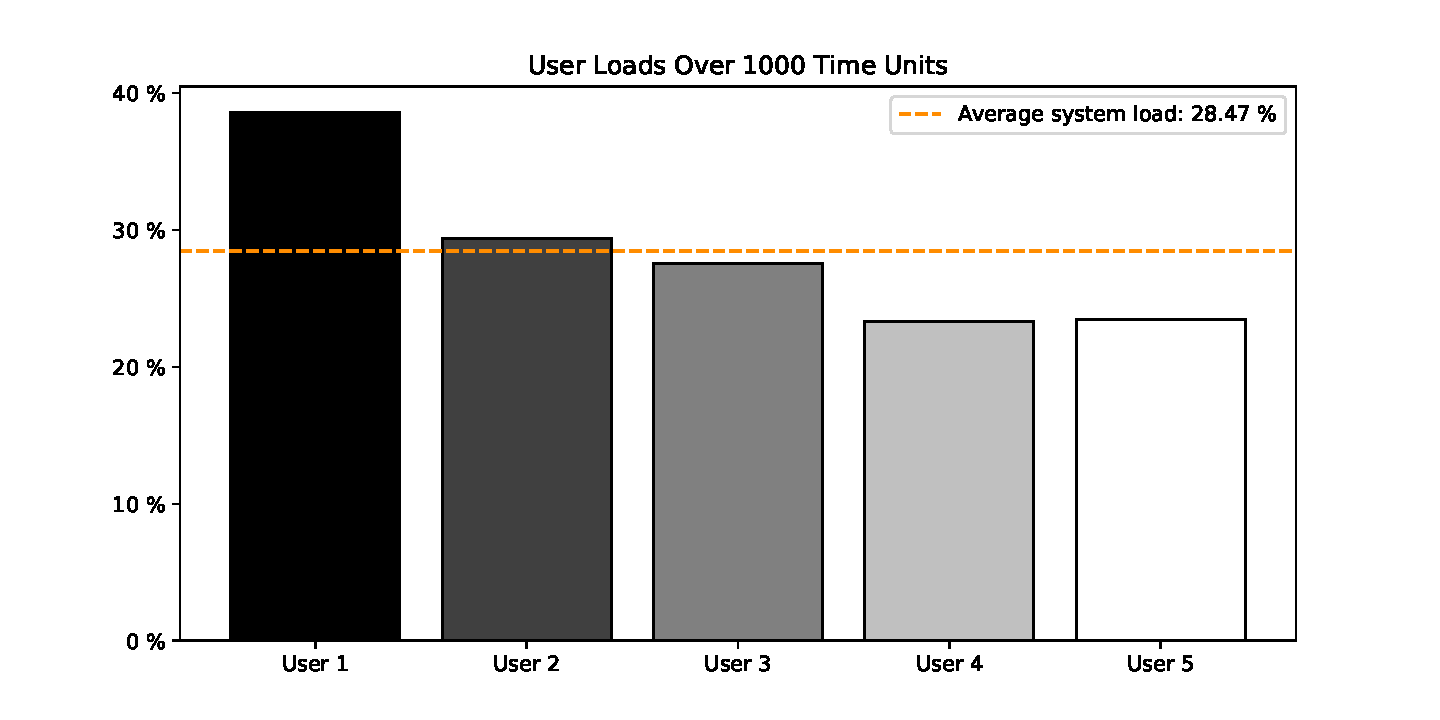
\includegraphics[width=\textwidth]{img/1_BATCHONE_MSA_NU5_GI3_SIM1000_FAIR}
		\caption{User loads distribution for 1-Batch-1 using \glsentryshort{msa}. More equally distributed histograms indicate fairer user treatement by the policy as seen in \figref{fig:st_fairness}.}
		\label{fig:msa_fairness}
	\end{minipage}
	\hfill
	\begin{minipage}[b]{0.45\textwidth}
		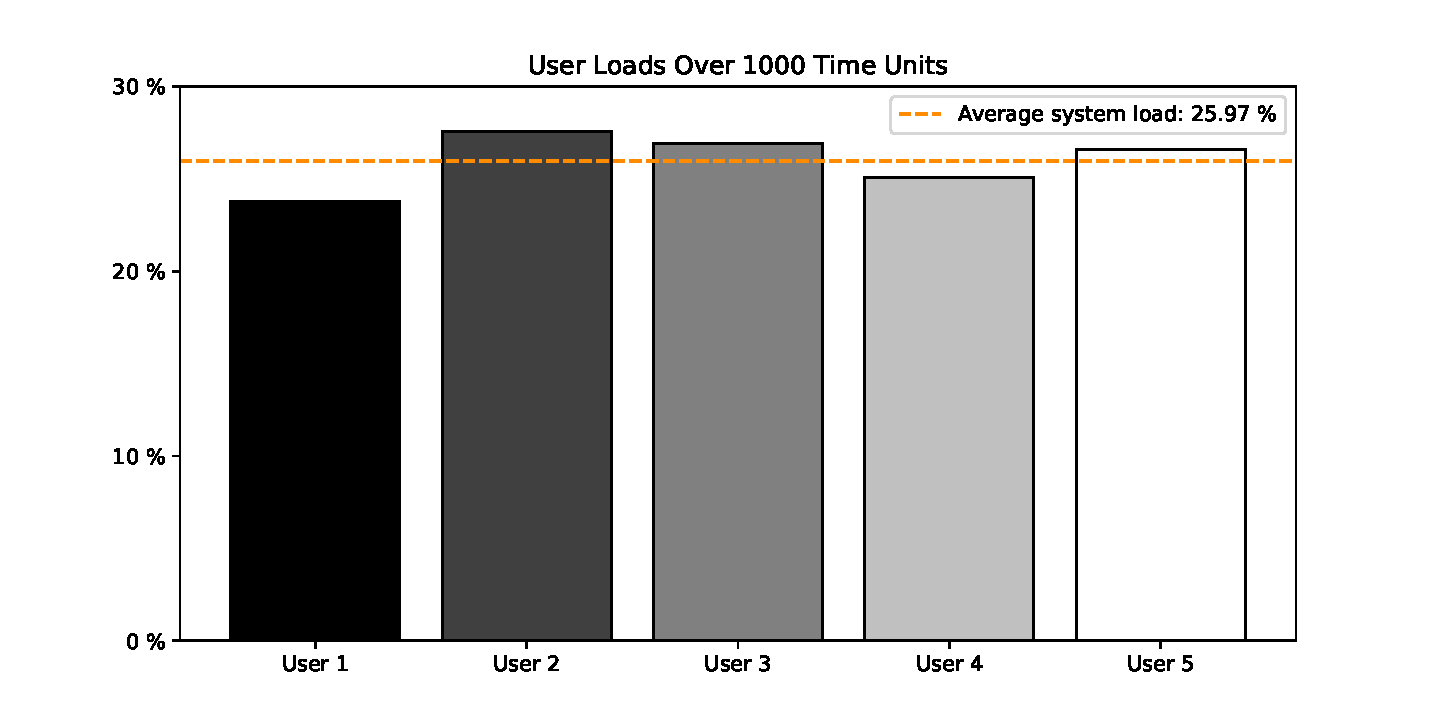
\includegraphics[width=\textwidth]{img/1_BATCHONE_ST_NU5_GI3_SIM1000_FAIR}
		\caption{User loads distribution for 1-Batch-1 using \glsentryshort{st}. More equally distributed histograms indicate fairer user treatement by the policy as seen here.}
		\label{fig:st_fairness}
	\end{minipage}
\end{figure}

Lastly, \gls{milp} based approaches solve role resolution in \glspl{wfms} in a deterministic way \ie they ``blindly'' optimize only at a specific point in time without accounting for the process dynamics. This kind of solution is done by the \gls{rl} methods outlined in \secref{sec:rl_discussion}.

\section{\glsentrylong{rl} Results Discussion}
\label{sec:rl_discussion}

Let us first focus on \gls{llqp}, which, as explained in \secref{sec:opt_policies}, focuses on assigning a job to the least loaded qualified person. By comparing the results obtained with \gls{rl} against the \gls{milp} based methods, we clearly see that speedups across all \glspl{kpi} are imperceptible (refer to \subsecref{subsec:llqp_rl_msa_comp_app} for more details). This sheds light on two key aspects:
\begin{enumerate*}
	\item \gls{llqp} policies are intrinsically optimized by their nature of implementation
	\item \gls{rl} methods converge really well\footnote{For a $1000$ time steps \gls{llqp} simulation, \gls{llqp} with \gls{td} and \gls{tf} only needs twenty times the simulation time as training in order to perfectly converge to actual \gls{llqp}.} and, even if only slightly, exploit internal mechanisms of \gls{llqp} policies to extract better results.
\end{enumerate*}

On the other hand, batch policies exhibit a much bigger optimization potential for which \gls{rl} methods do really adapt well. A $1.24$-fold speedup for 1-Batch (see \subsecref{subsec:onebatch_rl_msa_comp_app}) respectively $1.23$ for 1-Batch-1 (see \subsecref{subsec:onebatchone_rl_msa_comp_app}) confirm the previous claim.

Lastly, when accounting for job order during assignment (refer to \subsecref{subsec:batch_size_emulation} for the detailed explanation), improvements are observed only under specific conditions:
\begin{enumerate*}
	\item By using \gls{wzo} (see \figref{fig:wz_one_td_vfa_op}) 
	\item \glspl{ann} with \gls{1l} (see \figref{fig:bi_one_mc_tf_1l} for \glspl{kpi} comparison against \gls{msa} and \figref{fig:llqp_rl_ann_with_tf} for the graphical representation of the \gls{ann} implemented with \gls{tf}).
\end{enumerate*}

Having said that, deep \glspl{ann} exhibit worse results compared to their equivalent emulated \gls{milp} based methods. This can be explained from a twofold perspective:
\begin{enumerate*}
	\item \gls{vgp} which states that even very large changes in partial derivatives on initial layers have imperceptible effects on subsequent layers \citep{Bengio1994}
	\item \gls{egp} which states that huge spikes in the norm of changes in partial derivatives which could potentially grow exponentially can happen under training, thus influencing internal parameters \citep{Bengio1994,Pascanu2012}.
\end{enumerate*}

Yet another crucial aspect to consider when undergoing \gls{rl} methods is usage between \gls{onp} or \gls{op} learning (refer to \subsecref{subsec:onpol_pred} and \subsecref{subsec:onpol_control} for \gls{onp} respectively to \subsecref{subsec:offpol_methods} for \gls{op}). As shown in \tabref{tab:llqp_mc_vfa_op_vs_on} (and \figref{fig:llqp_mc_vfa_on_vs_off}), \gls{op} methods converge slightly better compared to \gls{onp}, however the change is imperceptible and can be found in different factors \eg random state seed choice or length of simulation. Having said that, it is important to note that these different approaches are being currently heavily studied by pioneers and the debate is still open, as \citet[pp. 245--249]{Sutton2017} explain. The current key takeaways from this outgoing debate can be summarized as follows \citep{Sutton2017}:
\begin{enumerate*}
	\item Learning \gls{op}
	\item Usage of scalable function approximation methods like linear semi-gradient 
	\item Usage of bootstrapping which is used in \gls{td} methods,
\end{enumerate*}
whose combination is referred to as ``the deadly triad'' \citep[p. 249]{Sutton2017}. \citet[p. 249]{Sutton2017} argue that dangers can arise only when all three aspects are present, if used singularly convergence properties are safe.

On a more general note, different comparisons have shown huge spikes in speedup of waiting time \eg as seen in \subsecref{subsec:onebatch_rl_msa_comp_app}. Even though compelling, the practical usage is limited: when considering \glspl{wfms} with fixed available resources \ie users participating, huge speedup in job waiting times does not always correlate with better system performance, since it might be the case that even if a job is ready to be assigned there are no available resources to complete such job.

\fig[\textwidth]{llqp_mc_vfa_on_vs_off}{\glsentryshortpl{kpi} comparison between \glsentryshort{op} and \glsentryshort{onp} approaches. Values bigger than $1.00$ indicate speedup while values smaller than $1.00$ indicate speeddown. Higher is not necessarily better (refer to \tabref{tab:llqp_mc_vfa_op_vs_on}).}{fig:llqp_mc_vfa_on_vs_off}

\section{Summary}
\label{sec:summary}

The focus of this thesis was analyzing different approaches for optimal role resolution in \glspl{wfms} by means of \gls{milp} and \gls{rl} based methods.

Initially, a through literature review has been made in order to establish the existing optimization solution \ie foundations set by \citet{Zeng2005}, then a roadmap on how to further develop such methods has been laid out. The roadmap encloses a twofold approach:
\begin{enumerate*}[ref=Approach \Roman*]
 	\item Further develop \gls{milp} based methods \label{itm:math_opt}
 	\item Use \gls{rl} methods as novel solution for role resolution in \glspl{wfms}. \label{itm:novel_rl}
 \end{enumerate*} 

Subsequently, a discrete event simulation environment as outlined in \chpref{ch:discrete_event_sim} has been implemented which served as foundation for evaluating all future optimization policies.

For \ref{itm:math_opt} five existing optimization policies as outlined in \secref{sec:opt_policies} have been implemented and evaluated against the existing policies defined by \citet[pp. 13--14]{Zeng2005}. Furthermore, for \ref{itm:novel_rl} a profound literature review about \gls{rl} had to be made and following on the theoretical foundations laid (see \secref{sec:rl_theory}), novel policies for solving role resolution in \glspl{wfms} based on \gls{rl} have been implemented (see \secref{sec:rl_policies}). Lastly, all \gls{rl} policies have been also evaluated and a comparison between them and the corresponding \gls{milp} methods has been made.

\gls{milp} based methods approach role resolution in a deterministic way \ie they optimize the assignment problem on fixed times without considering the dynamics of the system. The ``flagship'' formulation developed for this thesis, knows as \gls{st}, is a twofold optimization approach that outperforms traditional \gls{milp} based methods up to a $1.3$-fold speedup, but exhibits higher formulation complexity. 

\gls{rl} methods achieve the same results in term of speedup as \gls{st}. They additionally approach role resolution in a stochastic way, overcoming the deterministic drawbacks posed by traditional \gls{milp} based methods. Nonetheless, there are aspects that have to be accounted for when solving role resolution in \glspl{wfms} with \gls{rl} such as susceptibility of \glspl{ann} to \gls{vgp} and \gls{egp} when used as \gls{vfa}, lengthy training sessions required for convergence towards optimality and sensibility when using either \gls{onp} or \gls{op} learning.

\section{Consequences}
\label{sec:consequences}

\gls{milp} methods are viable solutions for role resolution in \glspl{wfms}, as already argued by \citet{Zeng2005}. Further developed policies relying on \gls{milp} done for this thesis proved indeed to yield better results (see \secref{sec:opt_results}), however the higher complexity required (refer to \secref{sec:optimization_discussion}) poses a critical trade-off. \ref{rq:one} can be affirmatively answer: there is definitely further development and optimization potential for traditional \gls{milp} based methods but further questions arise:
\begin{enumerate*}
	\item Does a slight increase in performance justify the higher formulation complexity requirements?
	\item Can only one \gls{kpi} be chosen as central parameter to evaluate a policy's performance or is a combination of different \glspl{kpi} more suitable?
	\item Is it always the best solution to use only one type of \gls{milp} based method or is it better to follow a more flexible approach and chose different policies on a per case basis?
\end{enumerate*}

All these questions must be accounted for when considering \gls{milp} based optimization methods to solve role resolution in \glspl{wfms}.

On the other hand, \gls{rl} methods demonstrate to overcome some of the problematics laid by optimization very well:
\begin{enumerate*}
	\item Generally less computationally expensive
	\item Can be adopted relatively fast
	\item Are generally more ``dynamic'' and can adapt and exploit case specific characteristics \ie overcome determinism of \gls{milp} based approached in favor of stochastic approaches.
\end{enumerate*}

Then again \gls{rl} methods are not exempt from disadvantages:
\begin{enumerate*}
	\item They require long training sessions in order to equal (or even outperform) optimization methods
	\item When using \glspl{ann}, overfitting might lead to suboptimal solution in which policies get stuck (for viable solutions refer to \citet{Srivastava2014})
	\item Multilayer \glspl{ann} \ie deep \glspl{ann}, are very sensitive to \gls{vgp} and \gls{egp} \citep{Bengio1994,Pascanu2012}.
\end{enumerate*}

In general \gls{rl} based approaches are a refreshing and novel methodology for solving optimization problems but require further development and sound domain knowledge.

\section{Outlook}
\label{sec:outlook}

This thesis sets the foundations for viable alternatives to existing \gls{milp} based techniques for role resolution in \glspl{wfms}. A direct follow up consists in testing in operative environments the introduction feasibility and efficiency of the methods measured in the discrete event simulation environment outlined in this thesis. This includes testing the robustness, efficacy and viability of the proposed policies by putting them under ``real-world'' stress situation in order to assert the speedup claims. For \gls{rl} methods executing lengthy training sessions might prove impractical: thousands of training sessions required by \gls{rl} methods in order to comply with convergence properties can prove infeasible for companies that are not able to generate such amounts of data, thus directly limiting applicability of these methods.

\gls{rl} is a novel field that is currently still being actively researched and pursued, as it has yielded promising results \citep{Mnih2015,Silver2016}. By using \glspl{ann} one can effectively approximate nonlinear functions as it has been outlined in \subsecref{subsubsec:ann_theory}. Even though in this thesis only feedforward \glspl{ann} have been used, the problem domain is very well suited for the recurrent variant as well.

Moreover, bleeding edge domains have originated from \gls{rl} such as \gls{irl} \citep{Ng2000} and \gls{al} which is based on the former \citep{Abbeel2004}. \gls{al} could prove to be yet another captivating approach to solve the assignment problem in which the reward function is not explicitly modeled, instead an ``expert'' of the domain \ie \gls{milp} based agents such as \gls{st} or \gls{msa}, demonstrates a task and by means of \gls{al} the policy is trained \citep{Abbeel2004}.

Having said that, \ref{rq:two} can be answered positively as well: there do indeed exist cutting edge approaches that can be used as alternatives or complements to role resolution in \glspl{wfms}. 